\section{Demonstration}\label{sec:demonstration}
%Our demonstration consist of using datasets from open data portals for some cities in France. \figref{expMappingParking} shows some of our experiments using these datasets. For each city, we performed two experiment. In \kword{NK}, no keywords are added by the user while in \kword{WK}, keywords are added. As we can see, even without keywords, there are fields that can be correctly mapped. Obviously, with keywords, initial mappings with better quality are generated. For all these datasets, we have their respective schema descriptions that we intend to use in our demonstration. 



%\begin{figure}
%	\centering
%	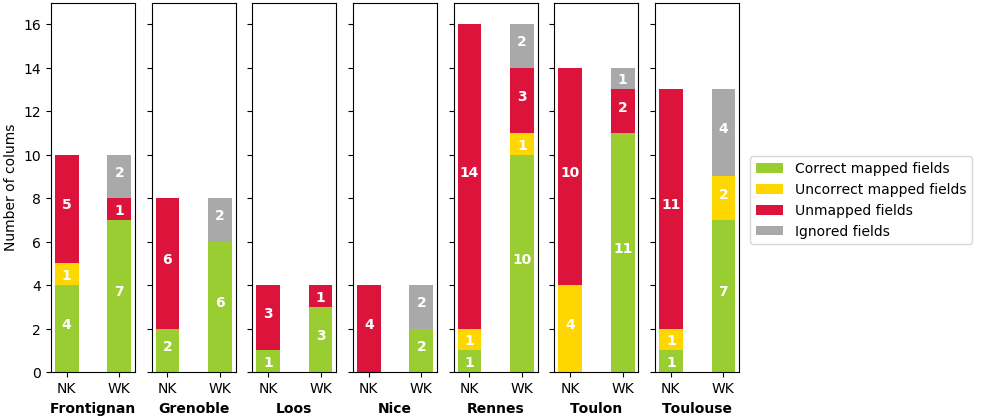
\includegraphics[scale=0.3]{./images/mappingPerParking1.png}
%	\caption{Mappings of the columns grouped per parking dataset. Where \emph{NK} represents the 
%		experiment without keywords and \emph{WK} represents the experiments with keywords.}
%	\label{fig:expMappingParking}
%\end{figure}

During this demonstration, we intend to RDFize Grenoble parking dataset partly shown in \figref{sampleRawData}. We perform two experiments: \kword{NK}and \kword{WK}. In \kword{NK}, we only specify the \kword{type description} with keywords. In \kword{WK}, we also specify keywords for interested columns. These keywords are shown in \tabref{overviewElementMappings}. Results are despicted in Table~\ref{tab:expGrenoble}. As we can see in \tabref{expGrenoble} and the video, adding keywords greatly improve the quality of mappings that are generated.

%\vspace{-0.5cm}

\section{Conclusion}
We have tested our approach on real datasets from open data portals and the results were promising. However, there are three main limitations. Firstly, the success of the approach depends much on the selection of keywords. It may not be easy for the user to define the keywords that will correspond to labels of ontologies entities. A extension of the approach that will suggest keywords according to these labels is currently being implemented. Secondly, as mentioned in \secref{approach}, our approach can consider raw data containing only one type of object described by several data properties. However in some cases, the object can be link in its description to other objets. Approaches dealing with entity resolution and entity linking could be used.  
Thirdly, as of now, there are no alignments between the ontologies in the ontology repository. The existence of these alignments can improve the quality of the generated mappings.



\begin{table}[]
    \centering
    \begin{tabular}{|c|c|c|c|c|c|c|}
        \hline
         &   LIBELLE & ADRESSE & TOTAL & id & lon & lat \\
        \hline
        NK & -- & schema:adress & --&  mobivoc:id & -- & -- \\
        \hline
        WK & schema:label & schema:adress & mv:Capacity & dc:id & geo:long & geo:lat \\
        \hline
    \end{tabular}
    \caption{Initial mappings without keywords (\texttt{NK}) and with keywords (\texttt{WK})}
    \label{tab:expGrenoble}
\end{table}
\vspace{-0.5cm}